%%%%%%%%%%%%%%%%%%%%
%%% Introduction %%%
%%%%%%%%%%%%%%%%%%%%
\section{Introduction}
\ac{RE} -i.e., the recovery of a model's geometric representation from potentially noisy and incomplete sensor data- is an important aspect of modern \ac{CAD} pipelines. 
It allows for convenient model editing based on real-world physical objects, thus simplifying and accelerating the product design process.
\\
An expressive and intuitive model representation scheme heavily used in solid modeling is \ac{CSG}.
It describes complex rigid solids by a binary tree with regularized boolean set-operations (eg. union, intersection, subtraction) as inner nodes and primitive solids (e.g. cubes, spheres, cylinders and cones) as leaves. 
This tree is also known as a model's Construction Tree.
\\
Due to the popularity of \ac{CSG} in \ac{CAD}, it is desirable to have tools at hand that are able to reliably recover a model's \ac{CSG}-tree from its point cloud representation stemming from sensor recordings.
\\
\ac{CSG}-tree generation might be solved by converting the input point cloud to a Boundary Representation (B-Rep) and then by conversion of the B-Rep to CSG with methods based on algorithmic geometry that usually require exact geometric intersection computations \cite{shapiro1993separation, buchele2004three}. 
These approaches are usually restricted to a single model representation for primitives, e.g. a surface description that uses quadrics. 
These methods can be also sensitive when handling inexact representations. 
\\
To overcome this constraint, \ac{CSG}-tree generation can be formulated as a combinatorial optimization problem over the possible permutations of primitives and set-operations for a fixed maximum \ac{CSG}-tree depth.
Metaheuristics, like \acp{GA} can then be employed for optimization \cite{mitchell1998introduction}.
\\
One of the most severe disadvantages of \ac{GA}-based solutions are computation times of minutes and hours for comparably small models ($\le 10$ primitives) \cite{fayolle2016evolutionary}.
This issue is addressed by the approaches proposed in this paper.  
\\
The basic idea of the described acceleration scheme is to exploit spatial relationships between primitives: 
Primitives that do not overlap spatially are not considered to be operands of a \ac{CSG}-operation.
This knowledge can be used to partition overlapping primitives and to compute partial per-partition results that are later on merged to a single \ac{CSG}-tree. 
\\
In particular, this paper makes the following contributions:
% in the field of \ac{GA}-based \ac{CSG}-tree recovery from point clouds: 
\begin{itemize}
\item An acceleration scheme based on spatial search space partitioning together with a robust merge mechanism.
\item A description and analysis of parallelization strategies for the proposed algorithms.
\end{itemize}  
The paper has the following structure: 
Section \ref{sec:relworks} discusses related work in the field of \ac{CSG}-tree extraction.
It is followed by an introduction of important concepts on which the paper is based on (Section \ref{sec:back}).
The problem to solve is detailed in Section \ref{sec:prob}.
The proposed solution is described in Section \ref{sec:concept} and evaluated in Section \ref{sec:eval}.
Section \ref{sec:conclusion} summarizes the results and sketches possible future work.
 
\copyrightspace

%%%%%%%%%%%%%%%%%%%%
%%% Related Work %%%
%%%%%%%%%%%%%%%%%%%%
\section{Related Works}
\label{sec:relworks}
This work is related to different domains such as surface reconstruction from discrete point clouds, reverse engineering of solid models or conversion from B-Rep to CSG. 
In this section, we briefly list some related works in these domains. 

\paragraph{Surface reconstruction}
The problem of reconstructing a surface from a discrete point cloud has been the subject of lots of attention in computer graphics. 
The most popular methods include fitting implicit surfaces such as \cite{OBATS03}, or Poisson surface reconstruction \cite{KH13} among others. 
The recent work of Berger et al. \cite{berger2017survey} presents a wide survey of the topic.
Using these methods, the reconstructed objects lack information that can be used for inspection or re-use of the object in further modeling. 

\paragraph{Reverse engineering, and B-Rep to CSG conversion}
The goal of reverse engineering is the creation of consistent geometric models from point cloud data \cite{VMC97,BMV01}. They usually output B-Rep models 
made of parametric patches.
\\
%\paragraph{B-Rep to CSG conversion}
The conversion from B-Rep to CSG was first investigated in 
two-dimension for linear polygons, then 
later extended by Shapiro for handling curved polygons \cite{shapiro1991efficient, shapiro2001convex}. 
The extension to three-dimensional objects was initially solved 
by Shapiro and Vossler in 
\cite{shapiro1991construction, shapiro1993separation} 
and later improved by 
Buchele and Crawford in \cite{buchele2004three}. 
These works rely on the fact that surfaces are composed of quadric surface patches. 
%(for computing separators, for factoring dominating halfspaces). 
One issue of these algorithms is that their worst time complexity can be 
exponential (the authors in \cite{buchele2004three} states a cubic 
time complexity in practice, while remarking that the worst time complexity could be exponential). 
Another issue is the handling of inexact representations. 
These methods work under the assumption that the patches form a clean partition of the 
target solid. However, in practice we are dealing with input point clouds that are potentially 
noisy, contain holes, or have additional details and thus the fitted primitives may not fit perfectly. 
This could impact the cellular classification on which these methods rely. 

\paragraph{Point cloud to CSG construction}
Close to our work are methods that handles noisy and incomplete point clouds 
such as \cite{schnabel2007efficient} for fitting primitives and methods that try to convert them to higher level representation such as \cite{fayolle2016evolutionary}. See also \cite[Sections~7 and 8]{berger2017survey} for further references. 
One of our goals in this work is to improve the running time of the evolutionary algorithm used in \cite{fayolle2016evolutionary} via geometric consideration (the overlapping in space of primitives).

%%%%%%%%%%%%%%%%%%
%%% Background %%%
%%%%%%%%%%%%%%%%%%
\section{Background}
\label{sec:back}
\subsection{Point Cloud to \ac{CSG}-Tree Pipeline} 
The extraction of a \ac{CSG}-Tree from a point cloud poses a complex problem which is usually solved with a processing pipeline that comprises the following steps:  
\begin{enumerate}
\item \textbf{Point cloud generation and pre-processing:} Point clouds are generated by laser scanners or tactile measurement devices. 
Other techniques use photogrammetric algorithms to gather depth information from (un-)calibrated camera images \cite{hartley2003multiple}.
Measured point clouds usually contain significant amounts of noise and outliers. 
These can be trimmed from the data-set using e.g. statistical approaches  \cite{rusu20113d}.
%\\
\item \textbf{Point cloud segmentation and primitive fitting:} The point cloud must be segmented and primitive parameters be fitted to the corresponding points. Approaches that fulfill both tasks for simple geometric shapes are e.g. specialized variants of the \ac{RANSAC} technique \cite{schnabel2007efficient}.
%\\
\item \textbf{\ac{CSG}-tree generation:} \ac{CSG}-tree generation can be done with methods based on algorithmic geometry such as \cite{shapiro1993separation, buchele2004three}, or via evolutionary approaches such as \cite{fayolle2016evolutionary} for handling inexact representations.
%\\
\item \textbf {\ac{CSG}-tree optimization:} The resulting \ac{CSG}-tree might not be optimal in terms of size and depth.
Additional optimization techniques can simplify the tree structure \cite{weiss2009geometry, shapiro1991construction}. 
\end{enumerate}

\subsection{Primitive Description}
Primitives are basic shapes located at \ac{CSG}-tree leaves. 
A primitive $p$ is fully described by its 
%totally differentiable 
signed distance function $f_p: \mathbb{R}^3 \mapsto \mathbb{R}$.
The surface of $p$ is implicitly defined by the zero-set of $f_p$: $\{x \in \mathbb{R}^3 : f_p(x)=0\}$.
Its surface normal at point $x \in \mathbb{R}^3$ is given by the gradient $\nabla f_p(x)$.
If the gradient does not exist at $x$ or is too expensive to compute, it can be approximated using the method of central differences:
\begin{equation}
\nabla f_p(x) \approx \frac{f_p(x - h) + f_p(x + h)}{2h},
\end{equation}
where $h$ is a small constant step size.

%\begin{figure}[htb]
%	\centering
%	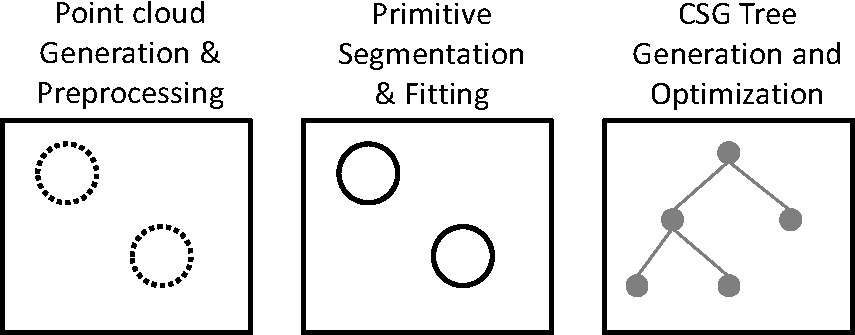
\includegraphics[width=0.5\textwidth]{figures/Praesentation1.pdf}
%	\caption{Insert caption to place caption below figure.}
%	\label{fig:spp}
%\end{figure}

\subsection{Boolean Set-Operations}
The set-operations intersection, union, complement and subtraction are implemented using $\min-$ and $\max$-functions \cite{ricci197constgeo}: 
\begin{itemize}
	\item Intersection: $S_1 \cap S_2 := \min(f_{S_1}, f_{S_2})$
	\item Union: $S_1 \cup S_2 := \max(f_{S_1}, f_{S_2})$
	\item Complement: $\overline{S} := -f_S$ %$\bar{S} := -f_S$
	\item Subtraction: $S_1 \setminus S_2 := S_1 \cap \overline{S_2}$% = max(-f_{S_1}, f_{S_2})$
\end{itemize}
where $S_i$ is the solid corresponding to the set $\{x \in \mathbb{R}^3: f_{S_i} \geq 0\}$ ($i=1,2$).
In the following, the considered boolean set-operations are $\{\text{intersection}, \text{union}, \text{subtraction}\}$.
\subsection{Evolutionary Algorithms} 
Evolutionary Algorithms are biology-inspired, stochastic metaheuristics for solving optimization problems.
\\
The optimization process starts with a randomly initialized population of individual candidates sampled from the problem's search space (initialization).
In each iteration, candidates are ranked according to their fitness by evaluating the so-called fitness function.
The best candidates are selected to be the next generation's parents (parent selection).
Parents are then recombined (crossover) and mutated (mutation) to create offspring. 
The new population is then filled with the offspring together with selected surviving individuals (survivor selection) from the current population.
This procedure is repeated until a certain termination criteria is met (termination). 
See Fig.~\ref{fig:evo} for an overview.
\\
Evolutionary Algorithms are especially useful for solving combinatorial optimization problems \cite{eiben2003introduction}.
%like the proposed formulation of the \ac{CSG}-tree extraction problem \cite{eiben2003introduction, fayolle2016evolutionary}.

\begin{figure}[htb]
	\centering
	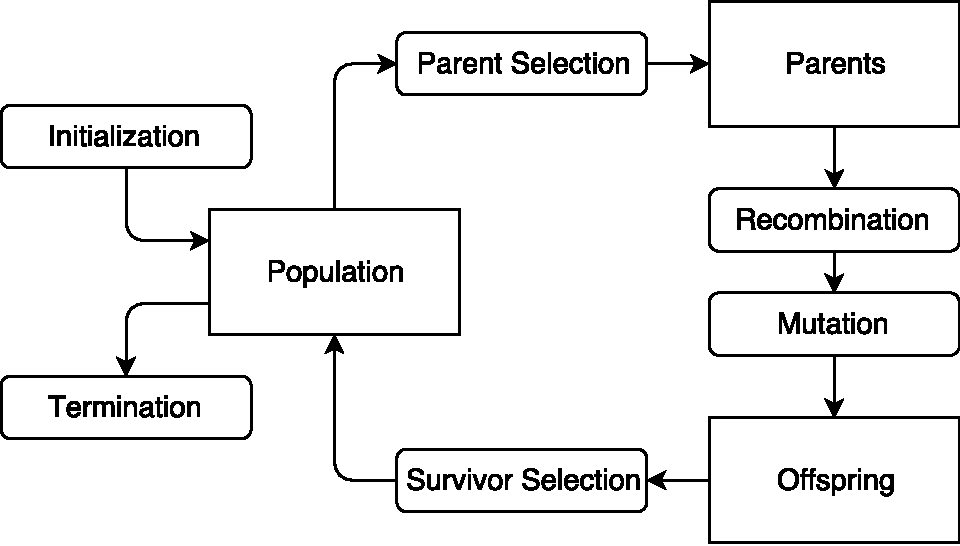
\includegraphics[width=0.45\textwidth]{figures/evo.pdf}
	\caption{The optimization process described by an Evolutionary Algorithm (derived from \cite{eiben2003introduction}).}
	\label{fig:evo}
\end{figure}

%%%%%%%%%%%%%%%%%%%%%%%%%
%%% Problem Statement %%%
%%%%%%%%%%%%%%%%%%%%%%%%%
\section{Problem Statement}
\label{sec:prob}
The problem of accelerating \ac{GA}-based \ac{CSG}-tree extraction from point clouds is considered as the open research question addressed by this paper.
\\
As input, a point-set of potentially noisy $3$-d measurements of a connected geometric model together with segmented and fitted primitives 
(and eventually separators \cite{shapiro1993separation}) 
is considered. 
The point-set might contain outliers and incomplete regions due to measurement errors that affect the result quality of the primitive reconstruction step.
\\
The desired output is a \ac{CSG}-tree that represents the scanned real-world model as accurately as possible.
\ac{CSG}-tree extraction approaches based on a \ac{GA} \cite{fayolle2016evolutionary} can handle 
inaccuracies but come with the disadvantage of high computation times.
%With each point, a position $p$ and its estimated normal vector $n$ is stored.  
%There is no further topological information given. 
%- Fehlerbehaftete und fehlende Punktwolken
%- CSG erstellen

%%%%%%%%%%%%%%%
%%% Concept %%%
%%%%%%%%%%%%%%%
\section{Concept}
\label{sec:concept}
The basic idea for \ac{GA} acceleration is to partition the search space in independent groups of spatially overlapping primitives.
This exploits the fact that primitives that do not overlap are not considered to be operands of a \ac{CSG}-operation.
\ac{CSG}-extraction is then conducted on a per-partition level. 
Finally, resulting trees are combined in a subsequent merge step without loss of result quality. 
\\
An overview of the full \ac{CSG}-extraction pipeline is depicted in Fig.~\ref{fig:pipeline_s}. 
Each of the steps is described in details in the following sub-sections, following the order of execution.

\begin{figure}[htb]
	\centering
	\begin{subfigure}[b]{0.3\linewidth}
		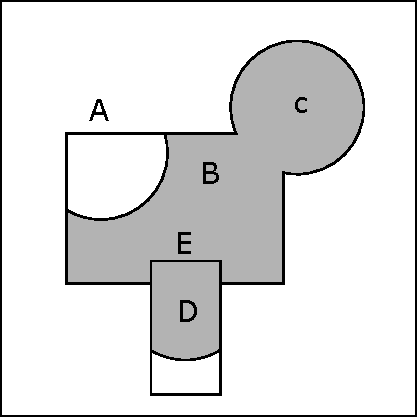
\includegraphics[width=\textwidth]{figures/pipe_0.pdf}
		\caption{Primitives.}
		\label{fig:pipe0}
	\end{subfigure}
	~
	\begin{subfigure}[b]{0.3\linewidth}
		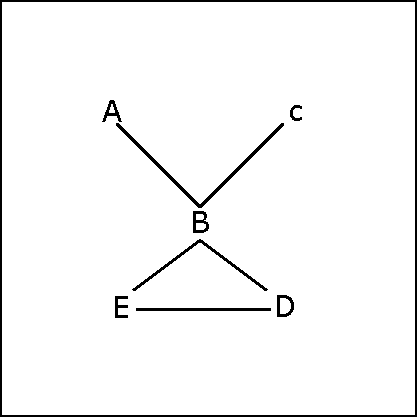
\includegraphics[width=\textwidth]{figures/pipe_1.pdf}
		\caption{\ac{PO}-graph.}
		\label{fig:pipe1}
	\end{subfigure}
	~
	\begin{subfigure}[b]{0.30\linewidth}
		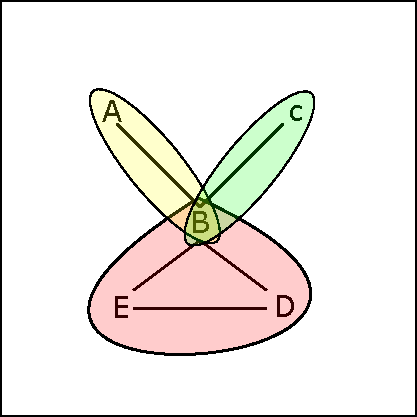
\includegraphics[width=\textwidth]{figures/pipe_2.pdf}
		\caption{Partitions.}
		\label{fig:pipe2}
	\end{subfigure}
	\vskip\baselineskip
	\begin{subfigure}[b]{0.633333\linewidth}
		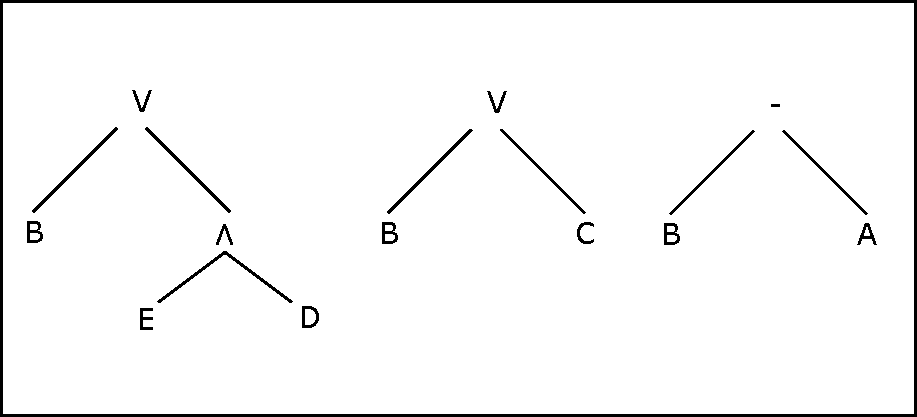
\includegraphics[width=\textwidth]{figures/pipe_4.pdf}
		\caption{Per-partition trees.}
		\label{fig:pipe3}
	\end{subfigure}
	~
	\begin{subfigure}[b]{0.30\linewidth}
		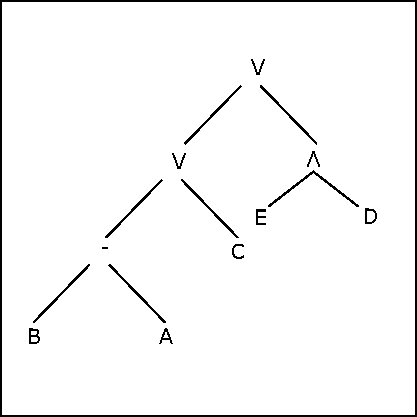
\includegraphics[width=\textwidth]{figures/pipe_3.pdf}
		\caption{Merged tree.}
		\label{fig:pipe4}
	\end{subfigure}
	\vskip\baselineskip	
	\caption{The search space partitioning pipeline.}\label{fig:pipeline_s}
\end{figure}

\subsection{Primitive Overlap Graph Generation}
\label{ch:pog}
For expressing spatial relationships between primitives, the \ac{PO}-Graph is introduced.
It represents spatial overlap between primitives using an undirected graph $G=(P,O)$, where $P = \{p_1,\dots,p_{n_p}\}$ is the set of $n_p$ primitives as vertices and $O$ is the edge-set that contains $2$-tuples of overlapping primitives $o=(p_i,p_j)$, where $i,j \in \{1,\dots,n_p\} \land i \ne j$. 
\\
The \ac{PO}-Graph is generated based on the location, orientation and geometric shape of the primitives, see Fig.~\ref{fig:pipe1} for an example.
Complex shapes can be approximated with simpler bounding volumes like \acp{OBB} or the convex hull of the corresponding point-set \cite{preparata1977convex}
\\
For better scalability, computational complexity can be reduced from $\mathcal{O}({n_p}^2)$ (overlap check between each primitive and each other primitive) to $\mathcal{O}(n_p\log(n_p))$ using hierarchical space partitioning schemes like Octrees \cite{meagher1982Octree}.
\subsection{Search Space Partitioning}
With known primitives and their spatial relations given by the \ac{PO}-graph, the goal is now to find independent search space partitions. 
\\
A partition is a set of primitives in which each primitive has an overlap with each other primitive.
In this context, independence means that per-partition solutions are not influenced by the solutions of other partitions.
See Fig.~\ref{fig:part} for explanatory examples. 
\\
The problem of finding all independent search space partitions is equivalent to the problem of finding all maximum complete subgraphs (maximum cliques) in $G$.
For finding the set of maximal cliques in $G$, the \ac{BKA}\cite{bron1973cliques} is employed due to its behavior on random graphs.
It was experimentally shown \cite{bron1973cliques} that the computational complexity of \ac{BKA} is almost independent of graph size for random graphs.
In a worst case scenario (using Moon-Moser Graphs \cite{moon1965cliques}), computational complexity is proportional to $(3.14)^{\frac{n}{3}}$, where $n$ is the size of the graph.
\\
Note that, if there is only a single partition for a particular \ac{PO}-graph, the search space partitioning method degenerates to standard \ac{GA}-based \ac{CSG}-tree extraction. 
The number of resulting partitions also depends on the accuracy of the hull approximation used for primitives during \ac{PO}-graph generation: 
The more inaccurate the approximation is, the less partitions will be created.

\begin{figure}[htb]
	\centering
	\begin{subfigure}[b]{0.3\linewidth}
		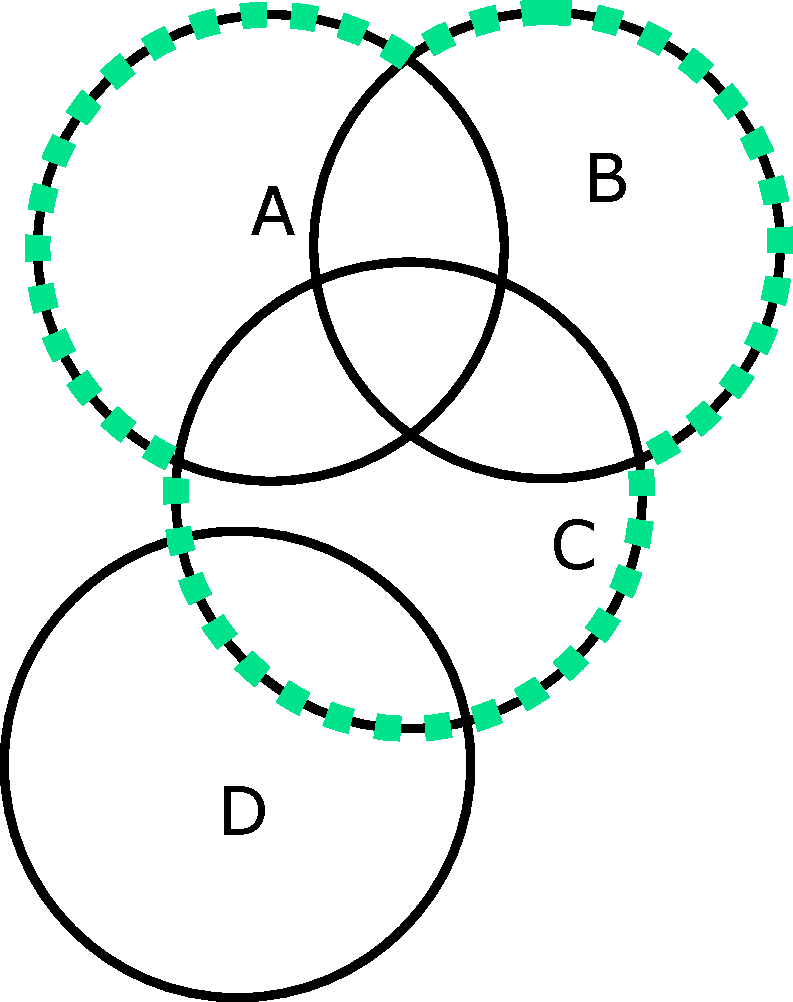
\includegraphics[width=\textwidth]{figures/right_part.pdf}
		\caption{correct}
	\end{subfigure}
	~
	\begin{subfigure}[b]{0.3\linewidth}
		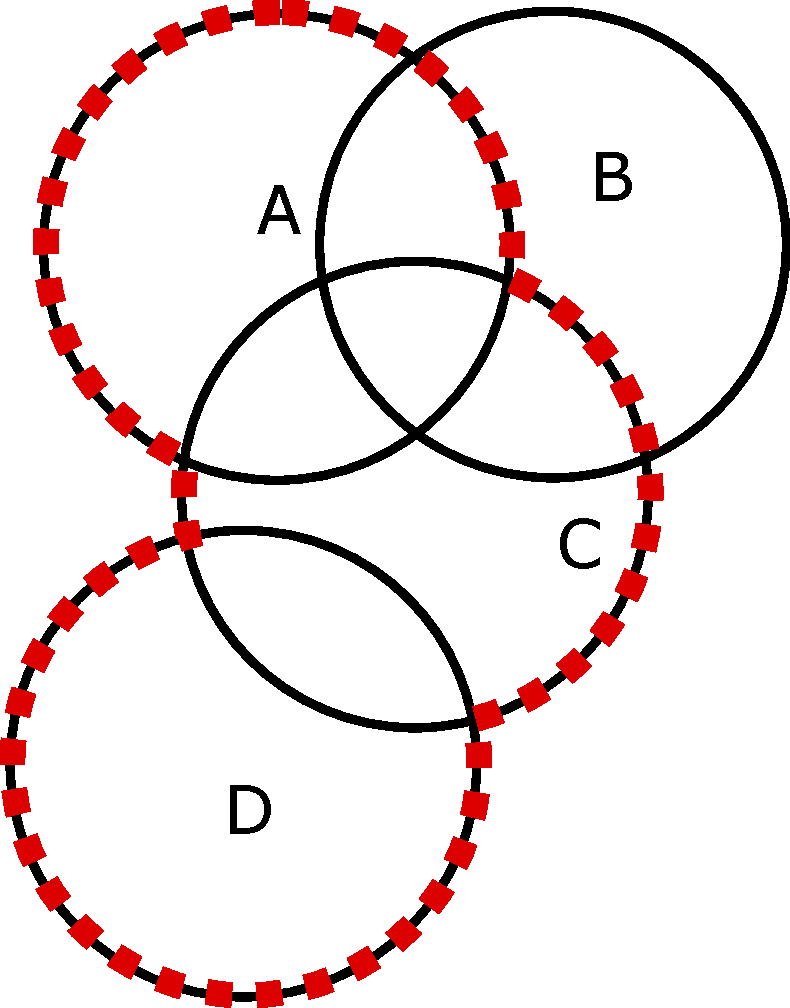
\includegraphics[width=\textwidth]{figures/wrong_part.pdf}	
		\caption{incorrect}
	\end{subfigure}
	\vskip\baselineskip	
	\caption{In the incorrect partition (red), B influences the per-partition solution without being part of the partition.}\label{fig:part}
\end{figure}

\subsection{Per-Partition \ac{CSG}-Tree Extraction}
\label{ch:ga}
With known partitions, \ac{CSG}-tree extraction is conducted for each partition separately in a divide-and-conquer manner.
%As a basic building block for all acceleration schemes proposed in this paper serves a variant of the \ac{GA} described in \cite{fayolle2016evolutionary} with the objective function
A variant of the \ac{GA} described in \cite{fayolle2016evolutionary} is used with the objective function
\begin{equation}
\label{eq:of}
E(t, S) := \sum_{i=1}^{|S|}\left\{e^{-d_i(t)^2}+e^{-\theta_i(t)^2}\right\}-\alpha \cdot \text{size}(t),
\end{equation}
where $t$ is the tree candidate, $S$ is the point-set and $\text{size}(t)$ is the number of nodes in tree $t$ weighted by $\alpha$.
$d_i(t) = \beta \cdot f_t(s_i)$ is the signed distance between point $s_i$ and the surface defined by tree $t$ weighted by $\beta$.
$\theta_i(t) = \gamma \cdot  \arccos(\nabla \hat{f_t}(s_i) \cdot n_i)$ is the angle between the point normal $n_i$ and the normalized gradient at position $s_i$ weighted by $\gamma$.  
$\alpha, \beta$ and $\gamma$ are user-controlled parameters. 
The first term in Equation \ref{eq:of} (under the sum) estimates how close the surface induced by $t$ matches the point cloud, while the second term penalizes trees with a large number of nodes.
%The third term penalizes large trees.
\\
Initially, the population $T_0$ is filled with $n_T$ randomly generated trees with a height $\le h_{max}$. 
For the maximum tree height, the approximation  
\begin{equation}
h_{max}\approx \sqrt{\pi \cdot \vert O \vert}
\end{equation}
is used, where $\vert O \vert$ is the size of the \ac{PO}-graph's edge-set.
It is based on the average height of binary trees for a given number of internal nodes \cite{flajolet1982TheAH} and worked well in all conducted experiments. 
\\
Each \ac{GA} iteration $i$ contains the following steps:
\begin{enumerate}
\item The population of the last iteration $T_{i-1}$ is ranked according to Equation \ref{eq:of}.
\item The current population is initialized with the $n_b$ best candidates from $T_{i-1}$.
\item As long as $T_i$ has not reached maximum population size $n_T$, two crossover candidates were selected from $T_{i-1}$ via Tournament Selection \cite{miller95genetic} parametrized with $k_{ts}$.
During crossover, the two candidates exchange randomly selected subtrees with a probability of $\gamma_{cr}$.
The resulting two trees are then mutated. 
In the mutation process a randomly chosen subtree is replaced with a new randomly generated subtree with a probability of $\gamma_{mu}$.
With a probability of $1-\gamma_{mu}$, the whole tree is replaced with a randomly generated tree.
\item The termination condition is met, if the score of the best \ac{CSG}-tree candidate of an iteration does not improve over $n_{tc}$ iterations.  	 
\end{enumerate}  
%The main difference of the described \ac{GA} variant compared to the \ac{GA} proposed in \cite{fayolle2016evolutionary} is the use of truncated solid primitives instead of implicitly defined surfaces of infinite extend in at least one dimension (eg. planes, cylinders). 
%This simplifies the algorithm since no additional limiting primitives must be introduced prior to extraction.
%\\
The most computational expensive step in \ac{GA}-based \ac{CSG}-tree recovery is the evaluation of Equation \ref{eq:of} for each element of a candidate-set. 
Since evaluations can be conducted for each candidate independently, parallel processing schemes can be efficiently applied.  
In addition, the solution space partitioning allows for an additional per-partition parallelization strategy.
Both options were implemented for multi-core processors and evaluated in Section~\ref{sec:eval}.
\subsection{Merge of Per-Partition Trees}
Merging all trees corresponding to partitions in a single tree is not trivial. 
A simple union of all tree root nodes leads to incorrect results if primitives that are part of multiple cliques are not splitted, see Fig.~\ref{fig:munion} for an example.
Split operations on arbitrary primitive shapes tend to be complex and thus should be avoided, see e.g. Fig.~\ref{fig:msplitting}.  
The proposed merge strategy does not need splits but instead tries to merge trees that have a common subtree.
It consists of the following steps:
\begin{enumerate}
	\item All trees are inserted in a list $L$ without adhering to any specific order.   
	\item The last two trees $t_0$ and $t_1$ are removed from $L$, and their largest common subtree $t_{lcs}$ is computed. The subtree's leaf-set must be a subset of the leaf-sets of $t_0$ and $t_1$. 
	A largest common subtree might exist more than once in both trees.
	Thus, the root nodes of each appearance of the subtree in $t_0$ and $t_1$ are stored in the lists $N_0$ and $N_1$.
	See Fig.~\ref{fig:subtree_0} for an example.
	\\	
	If $t_{lcs}$ is empty, $t_1$ is prepended to $L$ and a new tree candidate $t_1$ is removed from the end of $L$. This step is then repeated.
	\item For each node in $N_0$ and $N_1$ it is checked if it is a valid merge candidate.
	This is done by traversing the corresponding tree ($t_0$ or $t_1$) from root node to leaves following Algorithm \ref{al:trav}.
	If the node is reached that way, it is considered a valid merge candidate.
	The found merge node is then replaced by the root of the other tree resulting in a merged tree $t_m$.
	If more than one valid candidate exists, the candidate corresponding to the larger tree is replaced by the root of the smaller tree.
	If both trees are of the same size, the candidate of $t_0$ is chosen.  
	See Fig.~\ref{fig:subtree_1} for an example.
	\item $t_m$ is appended to $L$.
	\item The merge process is continued until there is only a single node left in $L$.
	Since the model to reconstruct is by definition connected, the merge process always terminates.
\end{enumerate}

\begin{figure}[htb]
	\centering		
	\begin{subfigure}[b]{0.6\linewidth}		
		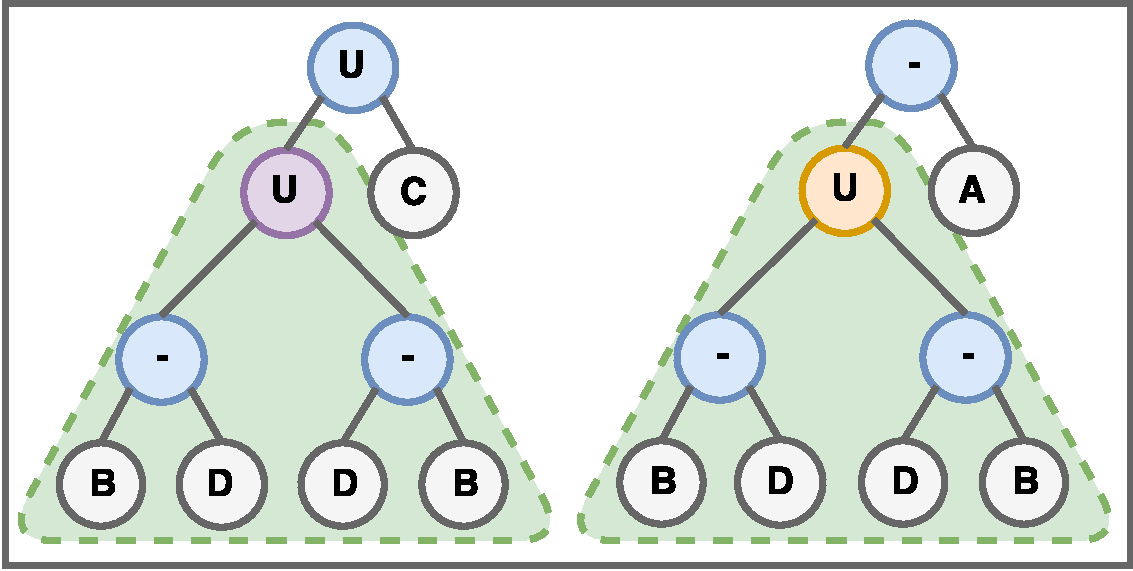
\includegraphics[width=\textwidth]{figures/subtree_0.pdf}	
		\caption{}			
		\label{fig:subtree_0}	
	\end{subfigure}
	~
	\begin{subfigure}[b]{0.3\linewidth}
		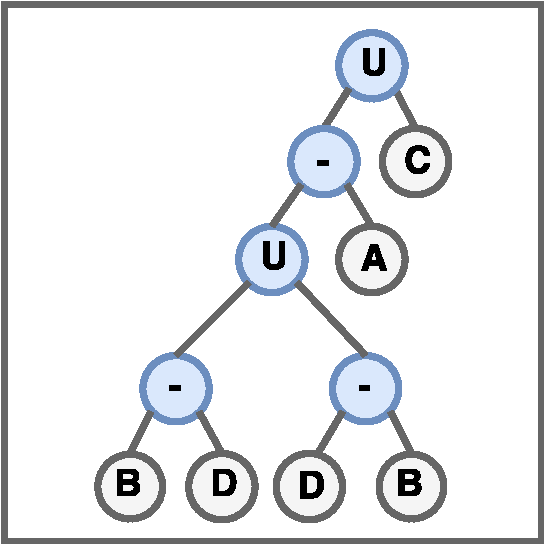
\includegraphics[width=\textwidth]{figures/subtree_1.pdf}
		\caption{}			
		\label{fig:subtree_1}
	\end{subfigure}	
	\vskip\baselineskip
	\caption{(\protect\subref{fig:subtree_0}) Two merge trees ($t_0$ left, $t_1$ right) with a largest common subtree (green). $N_0$ contains the purple node, $N_1$ the orange node. (\protect\subref{fig:subtree_1}) The merged tree $t_m$.}
\end{figure}

The merge process has an asymptotic computational complexity of $\mathcal{O}(\vert L \vert^2)$ since in the worst case $L$ has to be completely traversed for each merge.
Note that the proposed algorithm does not guarantee to find the $t_m$ with the minimal number of nodes possible. 

\begin{algorithm}[htb]
\SetKwProg{myproc}{Procedure}{}{}
\SetKwFunction{proc}{isValid}
\myproc{\proc{curNode, node}}{
	\uIf{curNode = node}{
		\KwRet {true}
	}
	\uIf{curNode.nodeType = Operation}{
		\uIf{curNode.operationType = Difference}{
			\KwRet {\proc{curNode.children[0]}}
		}
		\uElseIf{curNode.operationType = Union}{
			\ForEach{child $\in$ curNode.children}{
				\uIf{\proc{child}}{
					\KwRet {true}
				}
			}
		}	 	
	}	
	\KwRet {false}
}

\nl	\proc{$t$.root, node}
\caption{Checks if node \textit{node} is a valid merge candidate in tree $t$.}\label{al:trav}
\end{algorithm}
\begin{figure}[htb]
	\centering
	\begin{subfigure}[b]{\linewidth}
  		\centering
		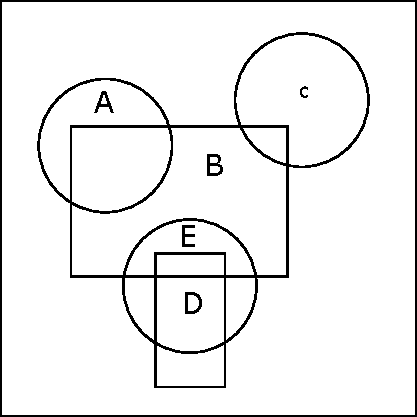
\includegraphics[width=0.6\linewidth]{figures/wm_0.pdf}
		\hfill
		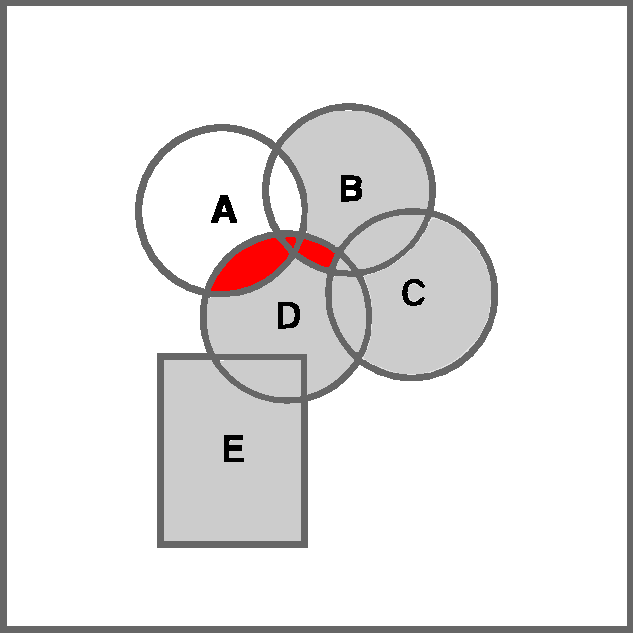
\includegraphics[width=0.3\linewidth]{figures/wm_1.pdf}
		\caption{Wrong tree merge using union over all partition trees. 
		Erroneous geometry in red (compare with Fig.~\ref{fig:pipe0}).}
		\label{fig:munion}
	\end{subfigure}
	\vskip\baselineskip
	\begin{subfigure}[b]{\linewidth}
		\centering
		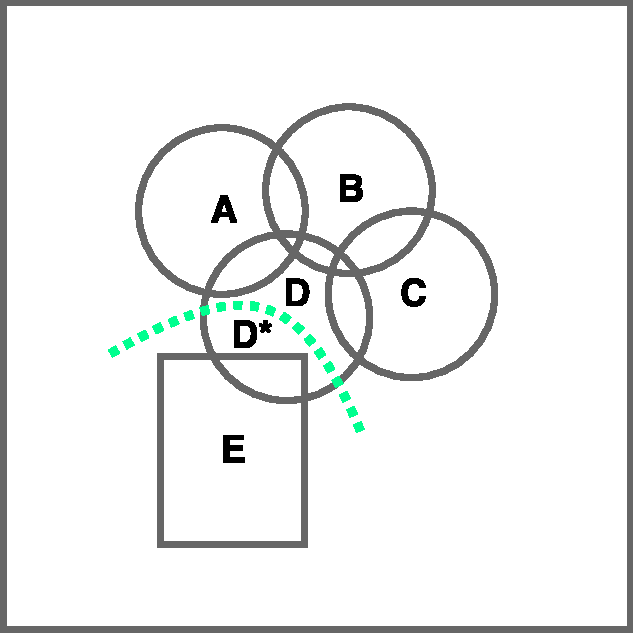
\includegraphics[width=0.3\linewidth]{figures/wm_2.pdf}
		\hfill
		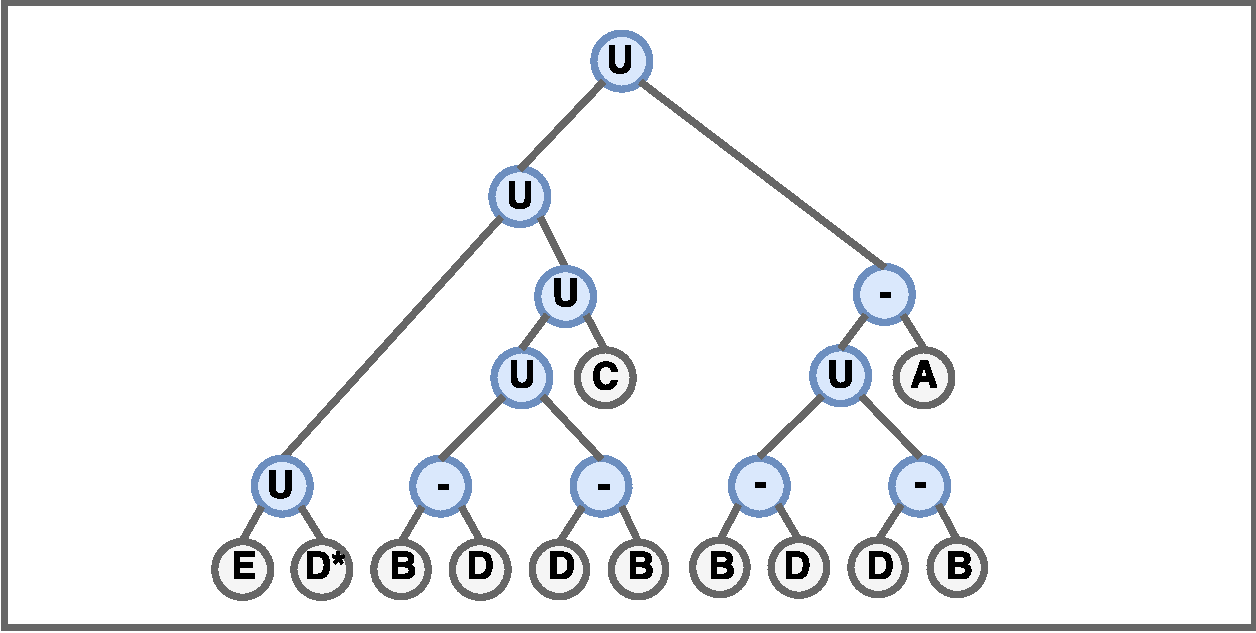
\includegraphics[width=0.6\linewidth]{figures/wm_3.pdf}
		\hfill
		\caption{Correct tree merge using union over all partition trees with primitive splitting (green curve).}
		\label{fig:msplitting}
	\end{subfigure}
	\vskip\baselineskip
	\caption{Merge strategies.}\label{fig:wmerge}
\end{figure}


%%%%%%%%%%%%%%%%%%
%%% Evaluation %%%
%%%%%%%%%%%%%%%%%%
\section{Evaluation}
\label{sec:eval}
The proposed partitioning scheme was evaluated on a laptop with quad core CPU and $16$GB of RAM on four different models.
For model $0$,$1$ and $2$, point clouds were generated by sampling a model surface induced by a pre-defined \ac{CSG}-tree that served as ground-truth. Gaussian noise was added to sampling points to simulate measurement errors.
Model $3$ is based on real measurements, and primitive fitting was conducted using RANSAC \cite{schnabel2007efficient}.
\\
The three synthetic models were sampled with different rates.
Table \ref{tab::models} contains model details. 
\begin{table}[h]
	\centering
	\begin{tabular}{|l|l|l|l|}
	\hline
	 & \textbf{M0} & \textbf{M1} \\
	\hline
	\# Primitives & 17 & 4  \\
	\hline
	\# Points (low) & 11.3k & 9.3k\\
	\hline
	\# Points (high) & 156.4k & 158.4k\\
	\hline
	\# Partitions & (0,8,4,0,1,1) & (0,0,2) \\
	\hline
	& \textbf{M2} & \textbf{M3} \\
	\hline
	\# Primitives & 29 & 18  \\
	\hline
	\# Points (low) & 10.9k & - \\
	\hline
	\# Points (high) & 155.4k & 55.8k \\
	\hline
	\# Partitions & (0,0,0,12) & (0,7,4,1) \\	
	\hline	
	\end{tabular}
	\caption{Details on evaluated models. 'low' and 'high' indicate different sampling rates. Numbers of partitions are depicted per partition size. First position in parantheses indicate number of partitions of size $1$ and so on.}
	\label{tab::models}
\end{table}
Baseline is the \ac{GA} approach proposed in \cite{fayolle2016evolutionary} and described in Section~\ref{ch:ga}. The parameter set used for both, baseline and partitioning scheme, is listed in Table \ref{tab:gaparams}.
\begin{table}[h]
	\centering
	\begin{tabular}{|l|l|}
		\hline
		\textbf{Parameter Name} & \textbf{Value}  \\
		\hline
		Population size $n_T$ & 150 \\
		\hline
		\# Best parents $n_b$ & 2 \\
		\hline
		Crossover probability $\mu_{cr}$& 0.3 \\
		\hline
		Mutation probability $\mu_{mu}$& 0.3 \\
		\hline
		Tournament selection parameter $k_{ts}$ & 2\\
		\hline
		Tree size weight $\alpha$& $\log(\text{\#points})$\\
		\hline
		Distance weight $\beta$& $100.0$ \\
		\hline
		Angle weight $\gamma$& $18.0/\pi$ \\
		\hline 
		\# Iterations w/o quality increase $n_{tc}$ & 10 \\
		\hline 
		Maximum tree height $h_{max}$ & $\sqrt{\pi\cdot \vert O \vert}$ \\
		\hline 
	\end{tabular}
	\caption{Parameters for the baseline and search space partitioning approach.}
	\label{tab:gaparams}
\end{table}
The following combinations were evaluated:
\begin{itemize}
	\item Baseline: Single-threaded (BST), multi-threaded \ac{GA} (BMTGA).
	\item Search Space Partitioning: Single-threaded (SST), per-partition multi-threaded (SMTP) multi-threaded \ac{GA} (SMTGA), per-partition and \ac{GA} multi-threaded (SMTPGA).
\end{itemize}   
\paragraph{Computation times}  
Timings for baseline and search space partitioning variants were measured for all models with high- and low-detail sampling (except for model $3$ for which only a single point cloud exists).
Measurements vary significantly for the same benchmark setting due to the inherently stochastic behavior of \ac{GA}-based methods. 
In order to deal with the high variance, each experiment was repeated $5$ times.
\\
In the following, timing results for all methods in combination with high-detail sampling are discussed.
For model $0$, SMTGA is the fastest method. 
It outperforms the baseline by a factor of $15.3$ (single-threaded, BST) and $7.5$ (multi-threaded, BMTGA) on average.
For model $1$, search space partitioning performs worse than baseline: 
The fastest baseline method (BMTGA) is on average $1.4$ times faster than the best-performing search space partitioning variant (SMTGA).
This can be explained by the relatively small number of primitives ($4$) and partitions ($2$) in model $1$ which eliminates the need for partitioning.
For model $2$, single-threaded partitioning is $38.3$ times faster than single-threaded baseline and multi-threaded partitioning variants are between $43.4$ and $46.6$ times faster than multi-threaded baseline.  
The considerable difference is due to the relatively high number of partitions ($12$) and their equally distributed size (all contain $4$ primitives).
For model $3$ SMTGA again is the fastest method. 
Compared to multi-threaded baseline it is $3.0$ times faster on average.
\\
Search space partitioning with \ac{GA} parallelization (SMTGA) is in general faster than their per-partition counterparts (SMTP, SMTPGA) for all models.
This is due to the granularity and regularity of the parallelization: 
For SMTGA, the task of ranking a population can be splitted in $n_T$ parts, with each part having similar execution times.
For per-partition variants, granularity is determined by the (potentially lower) number of partitions and per-partition execution times may vary a lot depending on partition sizes. 
\\
See Fig.~\ref{fig:graph1} and \ref{fig:graph4} for an overview of the results of the complete performance experiment.
Results for per-partition variants do not show timings for different pipeline steps since in all experiments, per-partition \ac{CSG}-tree extraction is by far the most dominant factor. 
The summarized time measures for \ac{PO}-tree generation, search space partitioning and tree merge make less then $1\permil$ of the total runtime.

\paragraph{Tree sizes and depths}  
Fig.~\ref{fig:graph2} contains average depths and sizes of resulting trees for baseline and partitioning variants.
For the latter, tree depths have increased by $50$-$155\%$ compared to the input tree, while for baseline approaches, an increase of only $0$-$80\%$ is visible.
Tree sizes show similar behavior:
Partitioning variants produce $57$-$77\%$ larger trees, while baseline approaches increase tree size by only $0$-$6\%$.
This adverse behavior of partitioning variants is due to the final merge step:
In each merge iteration, 
the two trees that are merged, are the neighbors in the merge list with a common subtree of at least size $1$, 
instead of the two trees with the largest common subtree. 
%not those two trees with the largest common subtree of all trees in the merge list are merged but those that are neighbors in the merge list and have a common subtree of at least size $1$.
Since the focus is on performance, this is acceptable.

\paragraph{Scalability with respect to point cloud size}  
Fig.~\ref{fig:graph3} depicts measurement results for the ratio
\begin{equation} \label{eq:ratio}
\frac{\#\text{points}_{high}}{\#\text{points}_{low}} : \frac{\text{duration}_{high}}{\text{duration}_{low}}
\end{equation}
which quantifies the dependency between point cloud size and corresponding computation times.
It indicates that, for larger models (model $0$ and $2$), the fastest partitioning approach scales up to $1.9$-times better than the best performing baseline approach with respect to point cloud size.
\begin{figure}[htb]
	\centering
	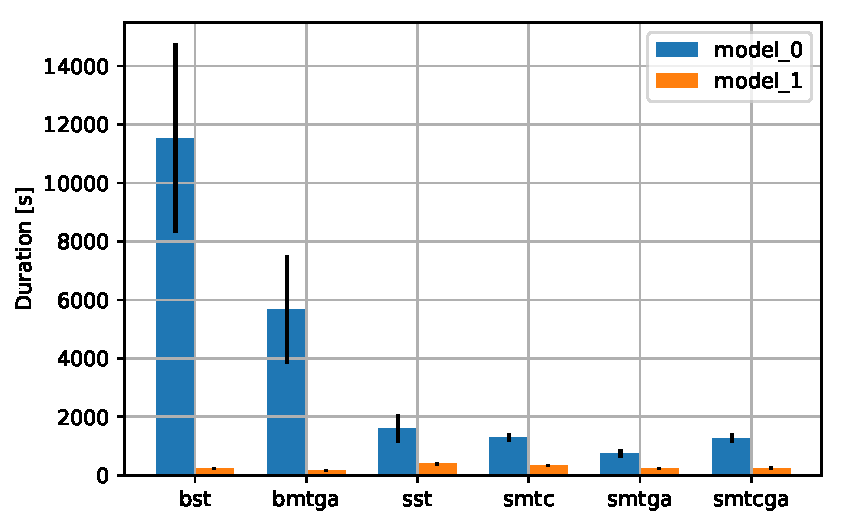
\includegraphics[width=0.5\textwidth]{figures/g1.pdf}
	\caption{Timings for all approach combinations and models $0$ and $2$ with high-detail sampling. Vertical black lines indicate standard deviation.}
	\label{fig:graph1}
\end{figure}
\begin{figure}[htb]
	\centering
	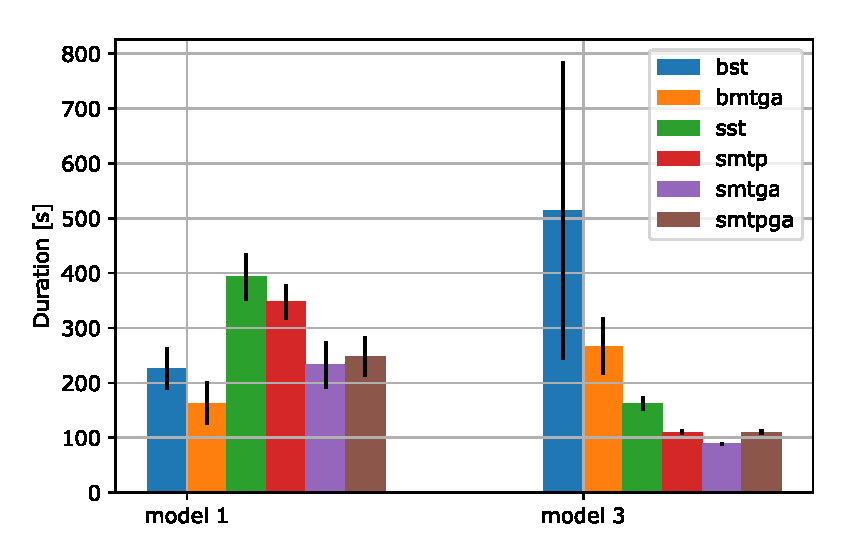
\includegraphics[width=0.5\textwidth]{figures/g4.pdf}
	\caption{Timings for all approach combinations and models  $1$ and $3$ with high-detail sampling. Vertical black lines indicate standard deviation.}
	\label{fig:graph4}
\end{figure}
\begin{figure}[htb]
	\centering
	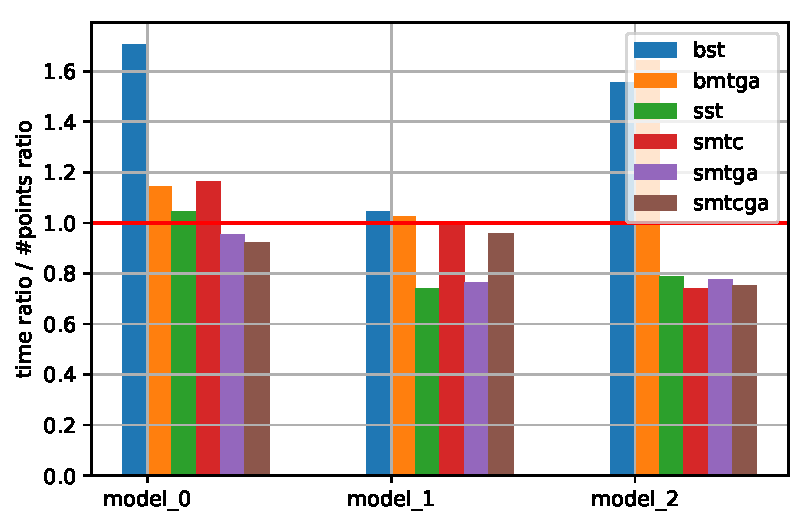
\includegraphics[width=0.5\textwidth]{figures/g3.pdf}
	\caption{Ratio between high-detail and low-detail point cloud size factor and corresponding timing factors for all models (see Equation \ref{eq:ratio}). The red line indicates linear scaling with a slope of $1$ with respect to point cloud size. Model $3$ is missing since it exists only in high-detail.}
	\label{fig:graph3}
\end{figure}

\begin{figure}[htb]
	\centering
	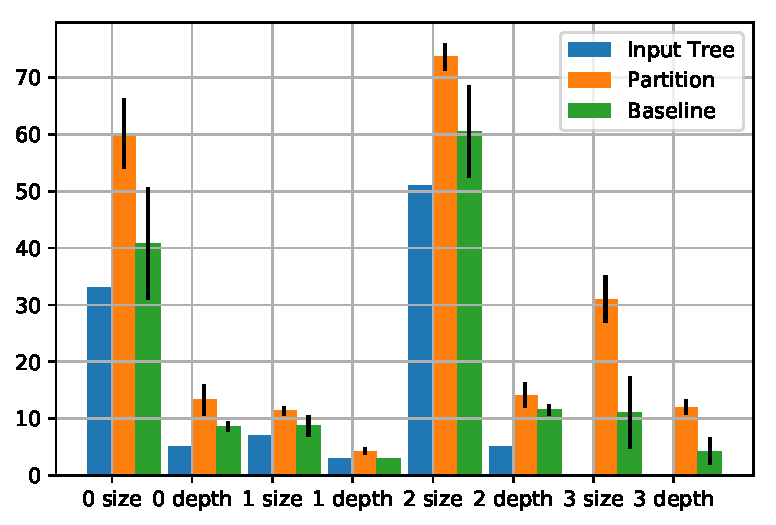
\includegraphics[width=0.5\textwidth]{figures/g2.pdf}
	\caption{Average tree size and depth for baseline and search space partitioning methods for all models with high-detail sampling. Vertical black lines indicate standard deviation.}
	\label{fig:graph2}
\end{figure}

	\begin{figure*}
		\centering
		\begin{subfigure}[b]{0.30\linewidth}
		\centering
		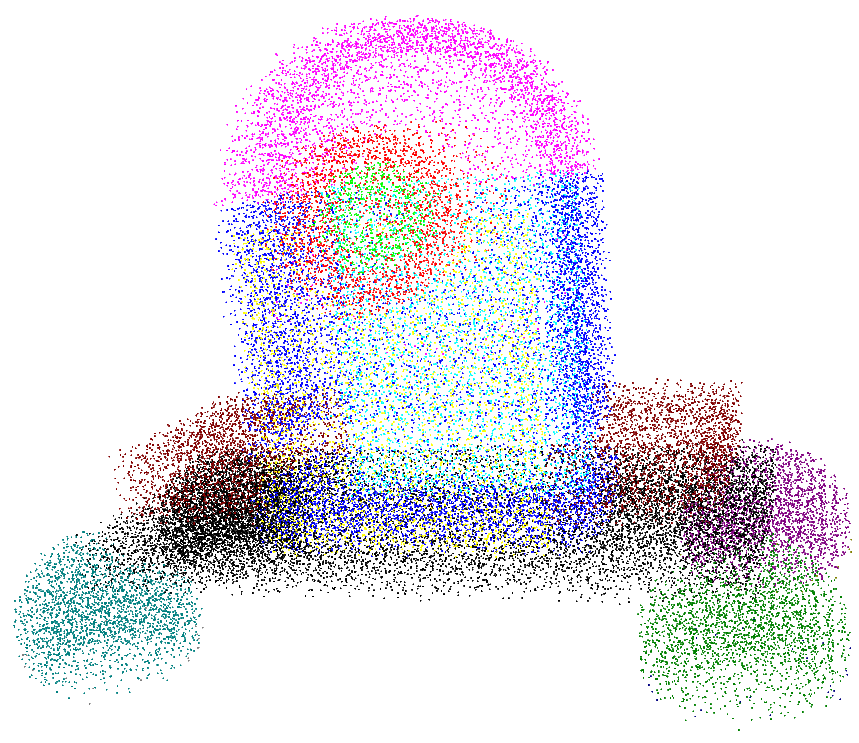
\includegraphics[width=\textwidth]{figures/m0_pc.png}
	\end{subfigure}	 
	\begin{subfigure}[b]{0.30\linewidth}
		\centering
		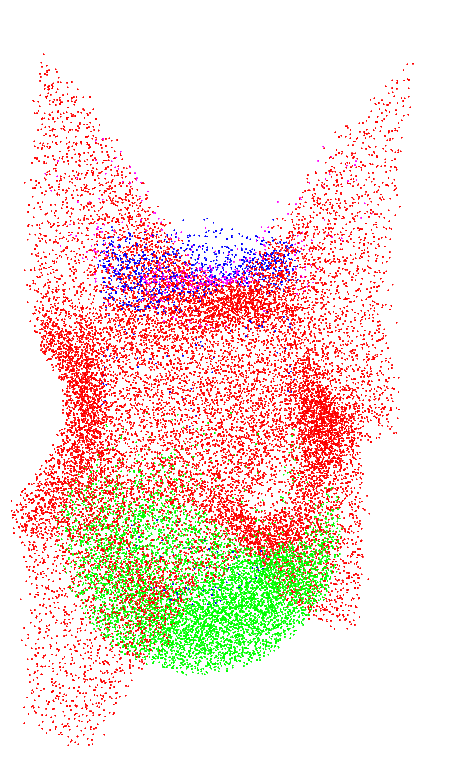
\includegraphics[width=\textwidth]{figures/m1_pc.png}
	\end{subfigure}	
	\\ 
	\begin{subfigure}[b]{0.30\linewidth}
		\centering
		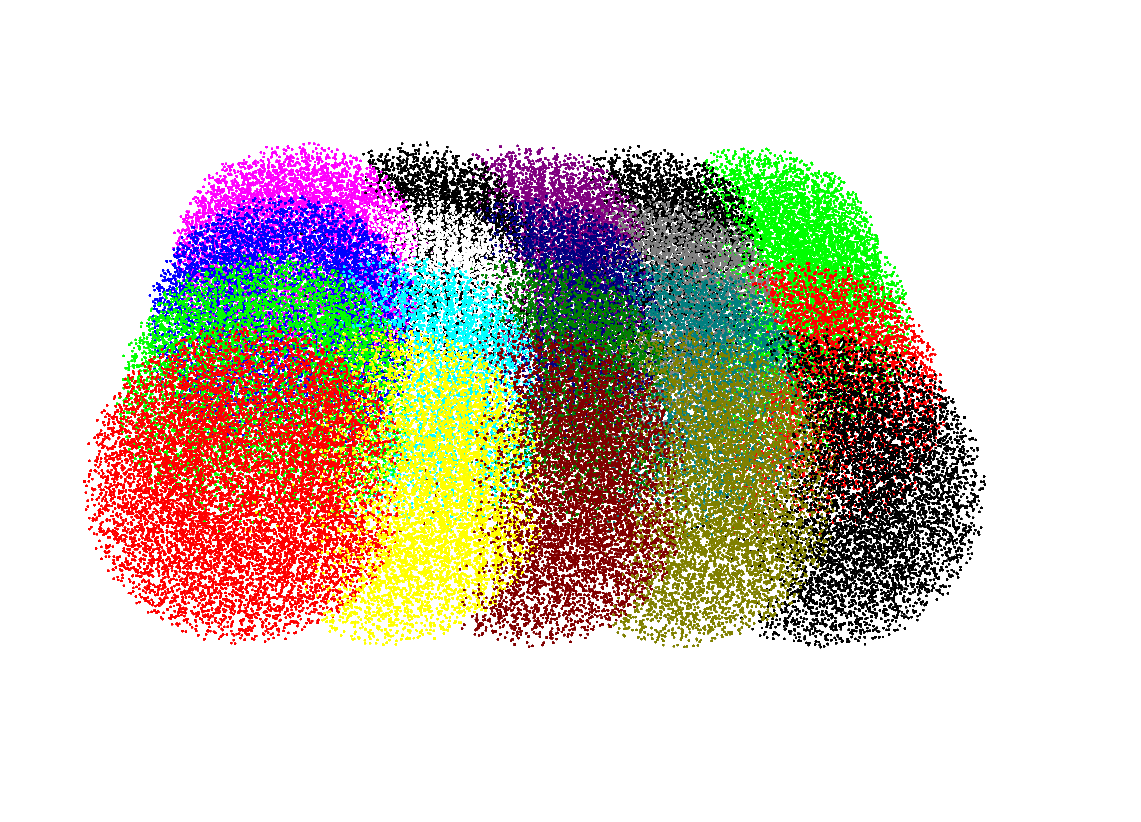
\includegraphics[width=\textwidth]{figures/m2_pc.png}
	\end{subfigure}	 	
	\begin{subfigure}[b]{0.30\linewidth}
		\centering
		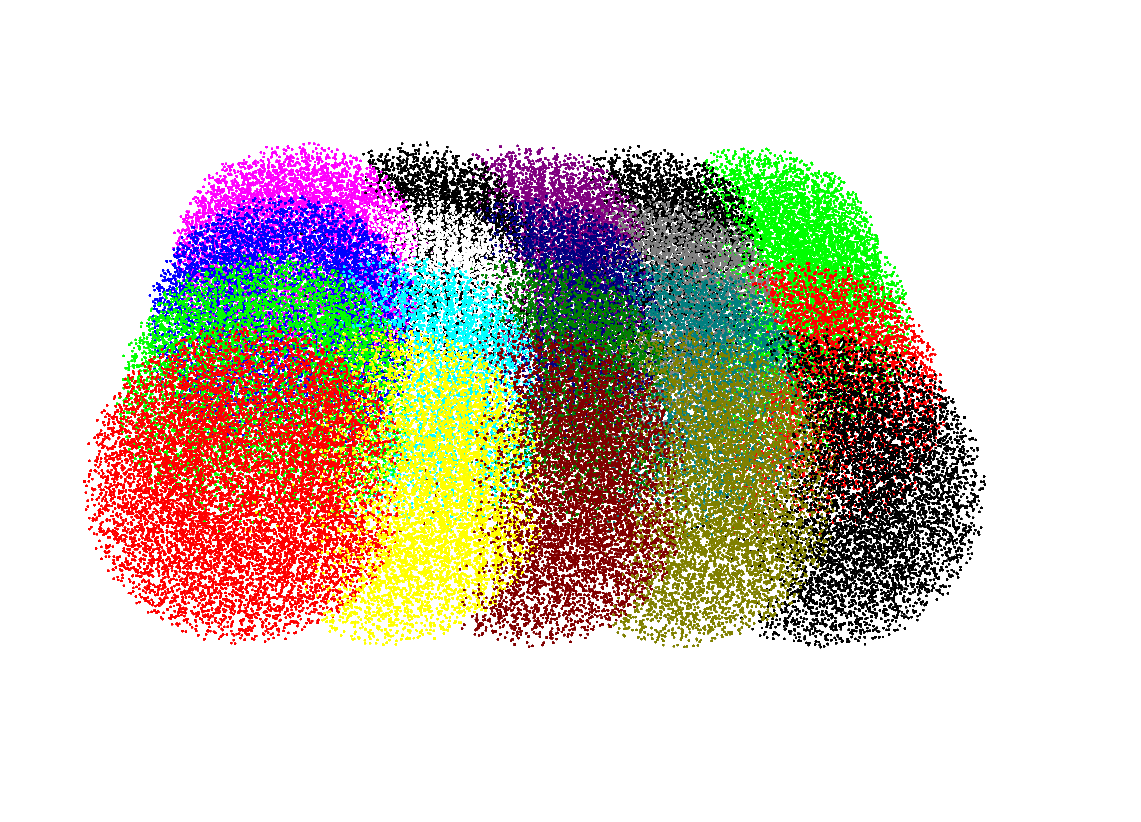
\includegraphics[width=\textwidth]{figures/m2_pc.png}
	\end{subfigure}	 
	\\
	\begin{subfigure}[b]{0.45\linewidth}
		\centering
		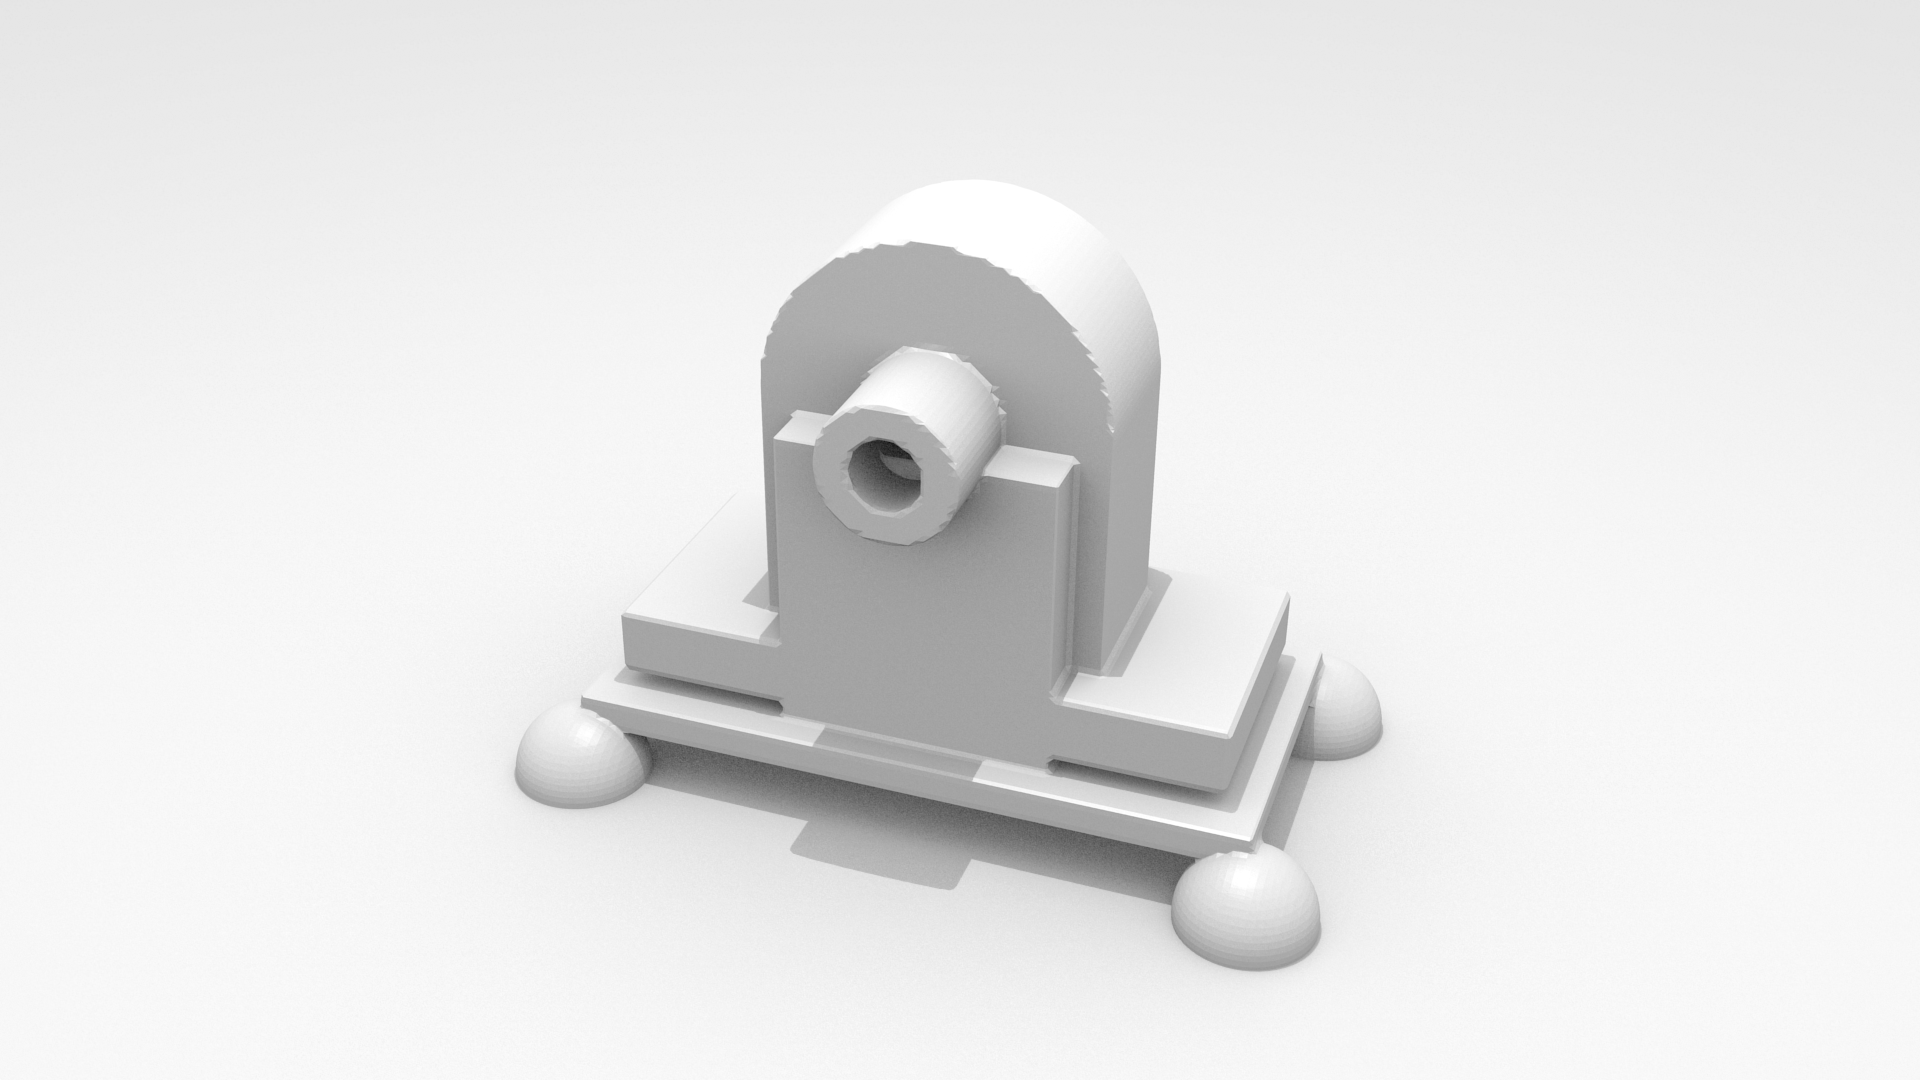
\includegraphics[width=\textwidth]{figures/m0_rendering.png}
	\end{subfigure}	 
	\begin{subfigure}[b]{0.45\linewidth}
		\centering
		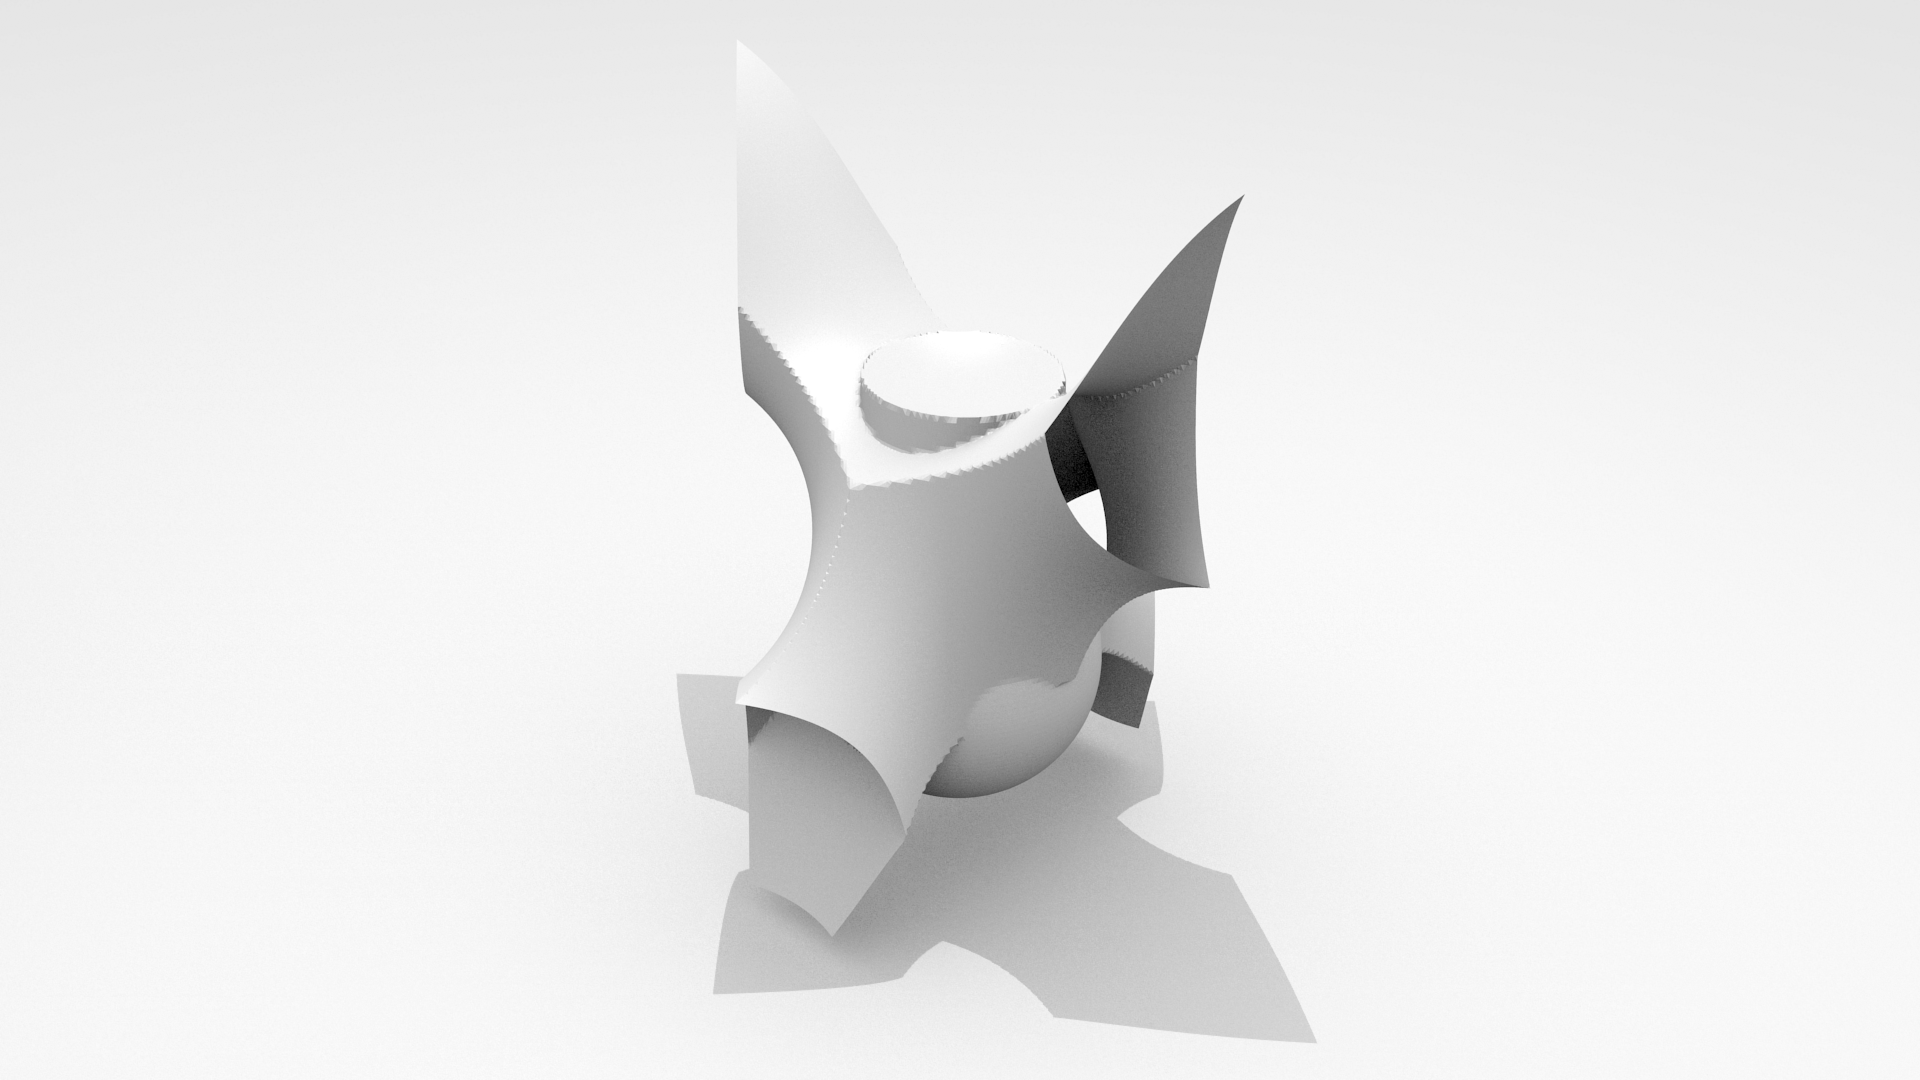
\includegraphics[width=\textwidth]{figures/m1_rendering.png}
	\end{subfigure}	
	\\ 
	\begin{subfigure}[b]{0.45\linewidth}
		\centering
		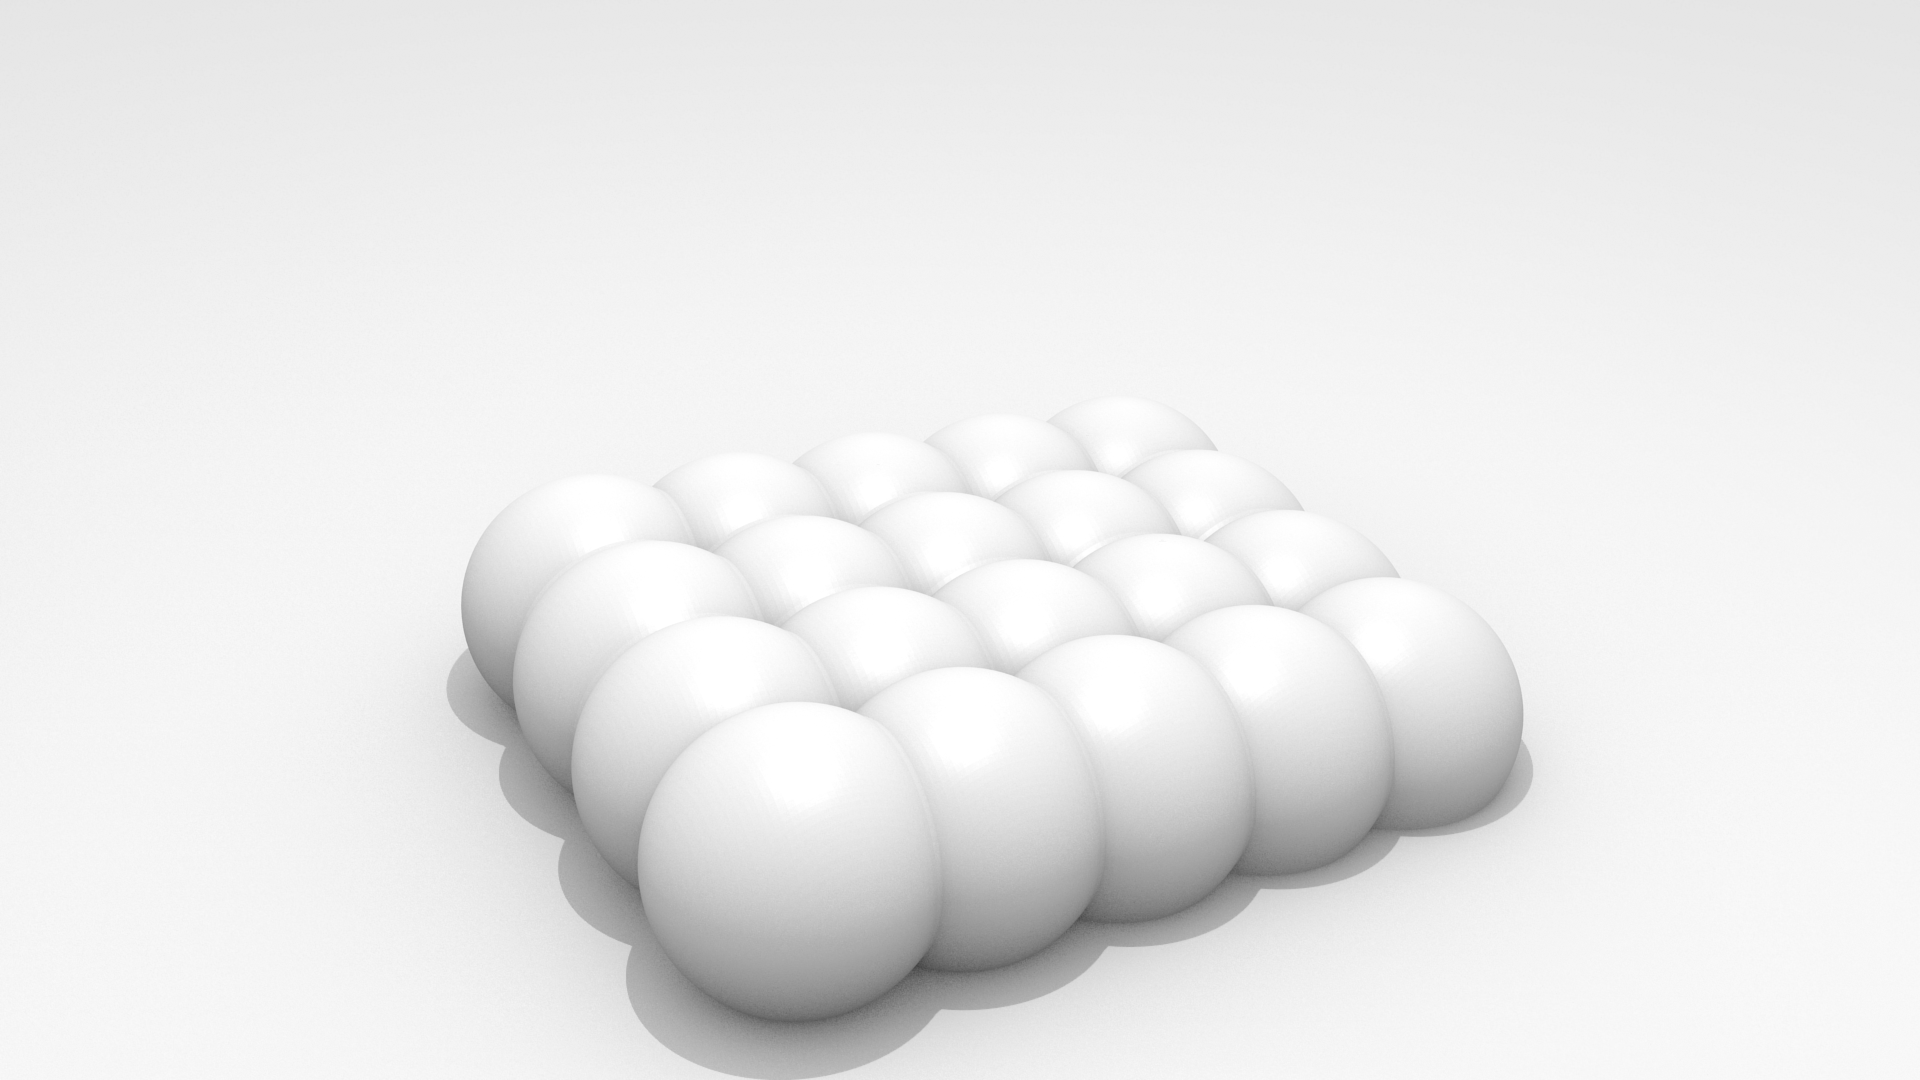
\includegraphics[width=\textwidth]{figures/m2_rendering.png}
	\end{subfigure}	 	
	\begin{subfigure}[b]{0.45\linewidth}
		\centering
		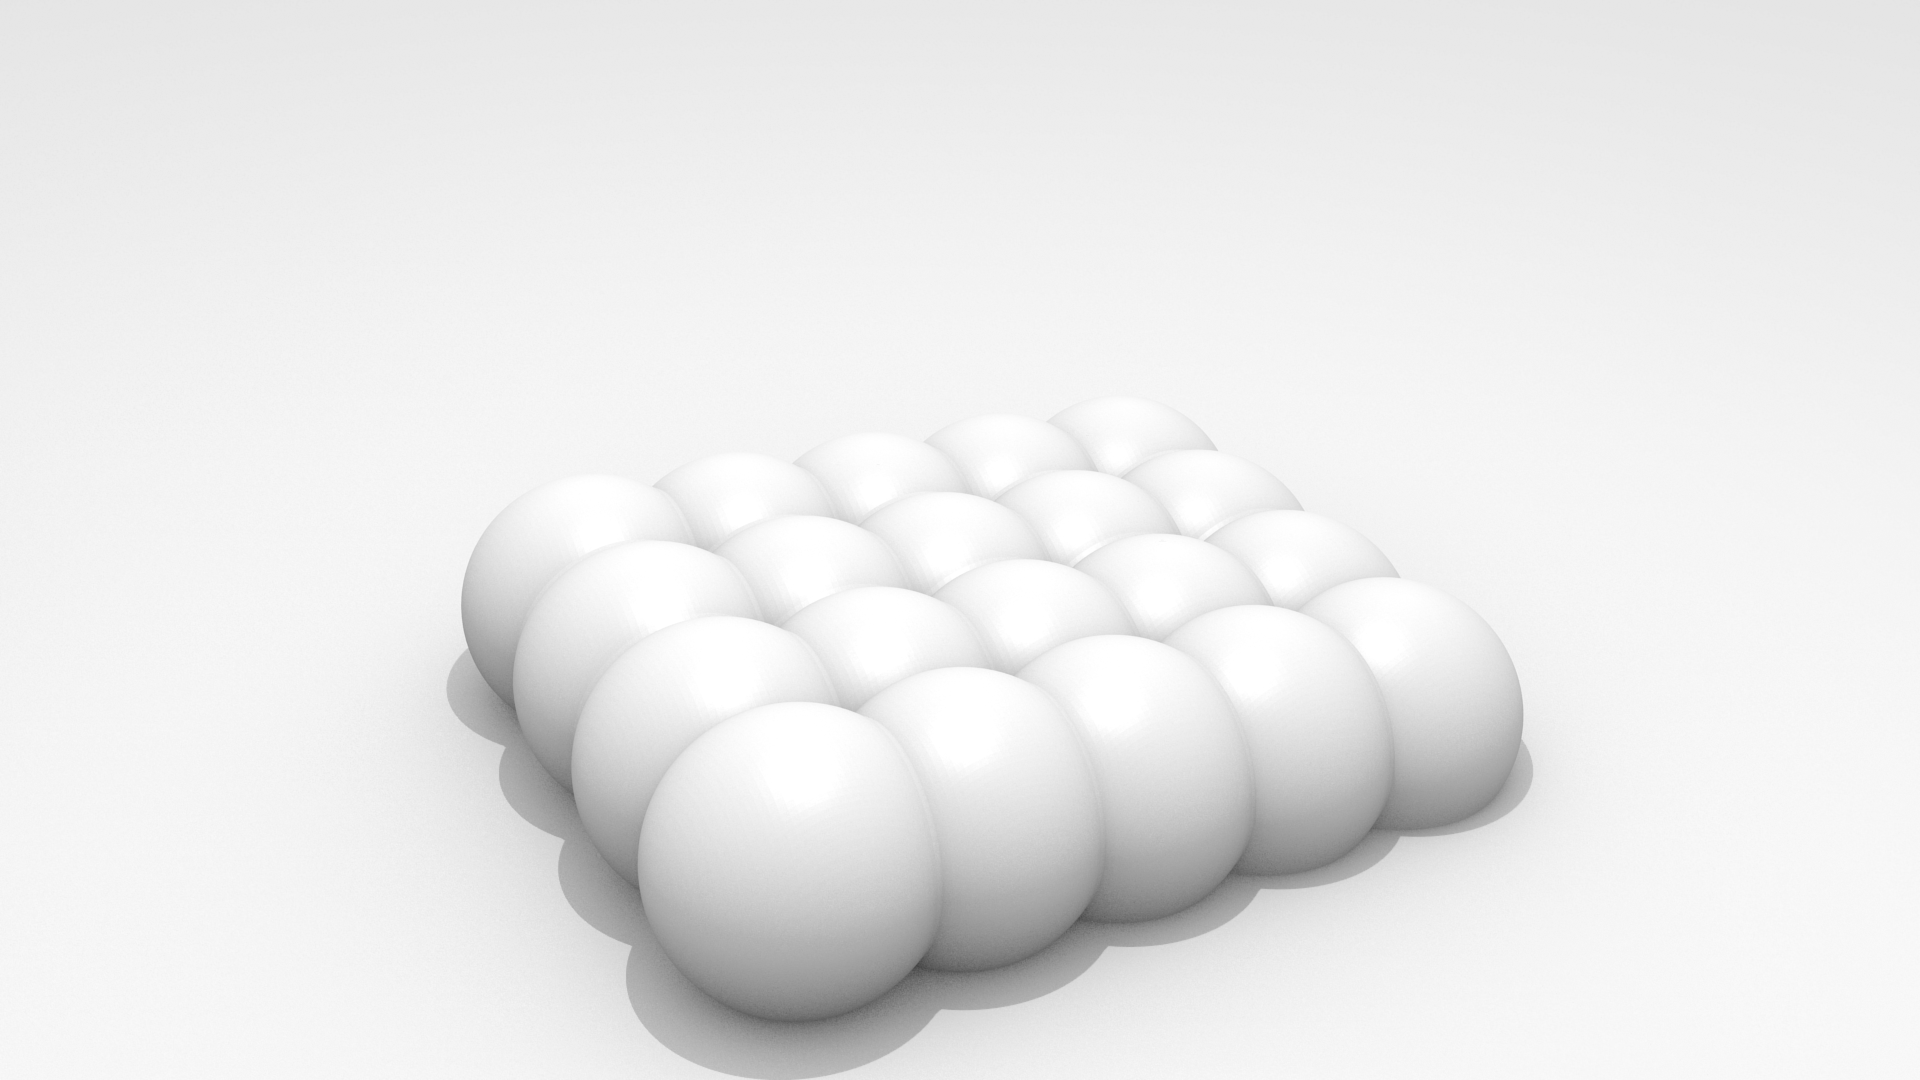
\includegraphics[width=\textwidth]{figures/m2_rendering.png}
	\end{subfigure}	 
	\caption{Point clouds and renderings of the resulting \ac{CSG}-tree representation of the models used in the evaluation.}
\end{figure*}

%%%%%%%%%%%%%%%%%%
%%% Conclusion %%%
%%%%%%%%%%%%%%%%%%
\section{Conclusion}
\label{sec:conclusion}
In this work a technique for accelerating an evolutionary algorithm for extracting 
a \ac{CSG} tree from a point cloud was proposed. Our method is based on a partitioning of the search space obtained 
from computing the maximal cliques of a graph of overlapping primitives, and on merging \ac{CSG} trees 
extracted for each partition. 
Our experimental evaluation indicated a significant speed-up over the baseline approach (the evolutionary algorithm) for different modes of parallelization.
\\
One possible direction for future works is 
the implementation of the \ac{GA} for massively parallel computing hardware, combined with the proposed partitioning approach. 
In addition, point cloud filtering based on sharp feature detection \cite{weber2010sharp} could further increase performance.
A decreased tree size in the partitioning approach could also be achieved by improving the merge process.
Finally, since the partitioning (and merge) approach described in this work is independent on the technique used for the CSG tree construction, the same approach could potentially be used with the CSG conversion approaches in \cite{shapiro1991construction,buchele2004three}. 
